%%%%%%%%%%%%%%%%%%%%%%%%%%%%%%%%%%%%%%%%%%%%%%%%%%%%%%%%%%%%%%%%%%%%%%%%%%%%%%%%
% Template for USENIX papers.
%
% History:
%
% - TEMPLATE for Usenix papers, specifically to meet requirements of
%   USENIX '05. originally a template for producing IEEE-format
%   articles using LaTeX. written by Matthew Ward, CS Department,
%   Worcester Polytechnic Institute. adapted by David Beazley for his
%   excellent SWIG paper in Proceedings, Tcl 96. turned into a
%   smartass generic template by De Clarke, with thanks to both the
%   above pioneers. Use at your own risk. Complaints to /dev/null.
%   Make it two column with no page numbering, default is 10 point.
%
% - Munged by Fred Douglis <douglis@research.att.com> 10/97 to
%   separate the .sty file from the LaTeX source template, so that
%   people can more easily include the .sty file into an existing
%   document. Also changed to more closely follow the style guidelines
%   as represented by the Word sample file.
%
% - Note that since 2010, USENIX does not require endnotes. If you
%   want foot of page notes, don't include the endnotes package in the
%   usepackage command, below.
% - This version uses the latex2e styles, not the very ancient 2.09
%   stuff.
%
% - Updated July 2018: Text block size changed from 6.5" to 7"
%
% - Updated Dec 2018 for ATC'19:
%
%   * Revised text to pass HotCRP's auto-formatting check, with
%     hotcrp.settings.submission_form.body_font_size=10pt, and
%     hotcrp.settings.submission_form.line_height=12pt
%
%   * Switched from \endnote-s to \footnote-s to match Usenix's policy.
%
%   * \section* => \begin{abstract} ... \end{abstract}
%
%   * Make template self-contained in terms of bibtex entires, to allow
%     this file to be compiled. (And changing refs style to 'plain'.)
%
%   * Make template self-contained in terms of figures, to
%     allow this file to be compiled.
%
%   * Added packages for hyperref, embedding fonts, and improving
%     appearance.
%
%   * Removed outdated text.
%
%%%%%%%%%%%%%%%%%%%%%%%%%%%%%%%%%%%%%%%%%%%%%%%%%%%%%%%%%%%%%%%%%%%%%%%%%%%%%%%%

\documentclass[letterpaper,twocolumn,10pt]{article}
\usepackage{usenix2019_v3}

% to be able to draw some self-contained figs
\usepackage{tikz}
\usepackage{amsmath, xspace}


% inlined bib file
%\usepackage{filecontents}
\usepackage{balance}

\newcommand{\needscitation}[1]{\textbf{\color{blue} NEEDS CITATION}}

\newcommand{\josh}[1]{\textbf{\color{red} Josh's Comment :: #1 }}
\newcommand{\peter}[1]{\textbf{\color{orange} Peter's Comment :: #1 }}

\newcommand{\sysname}{Kmap\xspace}

%-------------------------------------------------------------------------------
%\begin{filecontents}{\jobname.bib}
%%%%-------------------------------------------------------------------------------
%
%
%\end{filecontents}

%-------------------------------------------------------------------------------
\begin{document}
%-------------------------------------------------------------------------------

%don't want date printed
\date{}

% make title bold and 14 pt font (Latex default is non-bold, 16 pt)
%\title{\Large \bf Formatting Submissions for a USENIX Conference:\\
%  An (Incomplete) Example}

\title{Optimizing Envoy's Network Stack with \sysname}

 \author{
 {\rm Joshua Levin}\\
 Brown University
 \and
 {\rm Peter Cho}\\
 Brown University
 }

\maketitle
%\hypersetup{draft}

%%-------------------------------------------------------------------------------
%\begin{abstract}
%%-------------------------------------------------------------------------------
%KMap
%\end{abstract}

\section{Introduction}
\label{sec:introduction}
The development of the microservice and servicemesh has brought the sidecar container to the forefront of distributed services.
These sidecares provide shared features among services deployed on the servicemesh.
However, these sidecars are often interjected in a service-agnostic way by modifying iptables to redirect network communication through the sidecars.
This process can introduce significant latency to responses.
Istio has benchmarked Envoy to add between 5-10ms to response latencies on average for small to medium sized meshes (<=16 concurrent connections)~\cite{envoy_perf}.
We focus on the Envoy~\cite{envoy} sidecar used by the Istio~\cite{istio} servicemesh.

We present \sysname as an alternative library loaded via LD\_PRELOAD using shared memory to optimize data communication between processes.
Our work focuses on two key aspects:
\begin{enumerate}
    \item Building an efficient data path between Envoy and services
    \item Developing a robust API which mirrors classic POSIX sockets, which most common languages and tools use for interacting with the kernel stacks
\end{enumerate}

Our initial prototype explores challenges and design paths for the development of \sysname~\cite{kmap_source}.
We highlight challenges for implementing \sysname for production network systems.
Then, we present our prototype working on sample C/C++ webservers.
\section{Background}
\label{sec:background}
Recent shifts to microservice architectures and the resulting servicemesh have prioritized development and deployment efficency over performance.
Microservices deployed on a servicemesh (i.e. Istio~\cite{istio}) use proxies which are co-located with microservices.
These proxies intercept and control networking communication between services.
The proxies are relatively lightweight, but use the networking stack for communication with the co-located service (Figure-\ref{fig:no_kmap}).
They do this to preserve a common interface for services-- the networking stack.
Istio uses Envoy~\cite{envoy} which is the tool we focus on here for \sysname.
\begin{figure}[!htb]
    \begin{minipage}{0.5\textwidth}
        \centering
        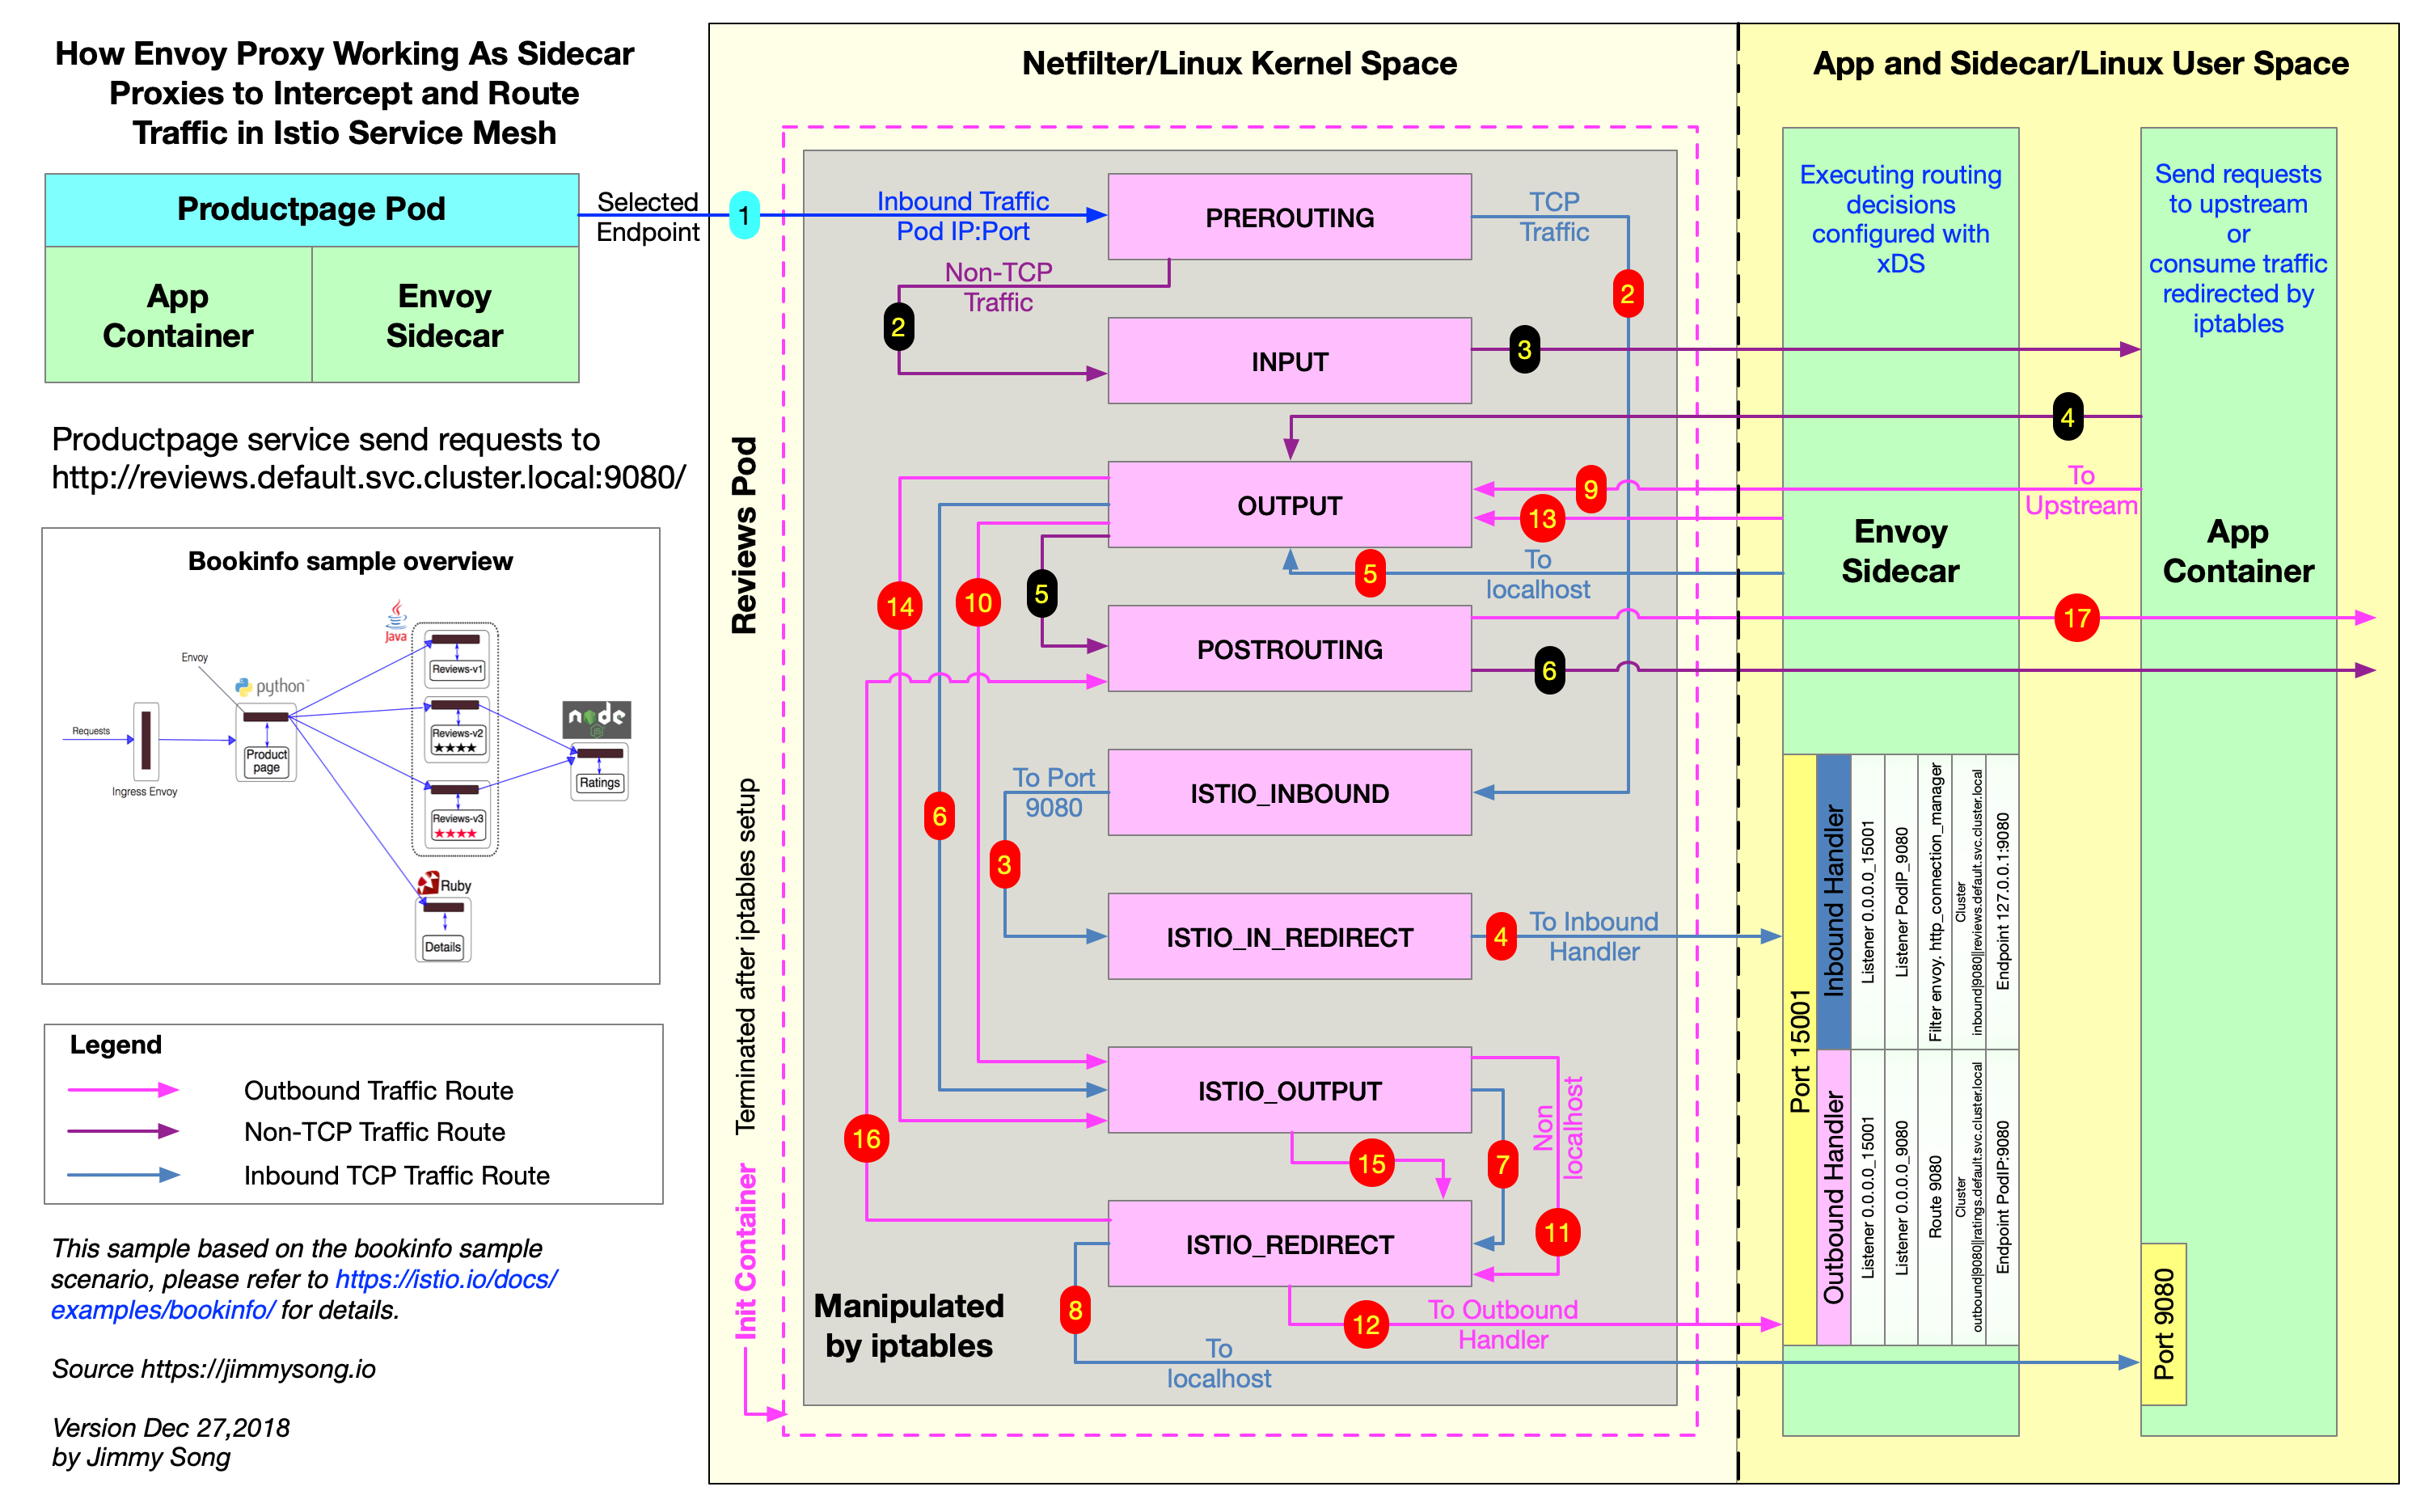
\includegraphics[keepaspectratio=true,width=3in]{figures/background/envoy.png}
        \caption{Envoy Network Stack~\cite{envoy_image}}
        \label{fig:envoy}
    \end{minipage}%
\end{figure}


\begin{figure*}[!htb]
    \begin{minipage}{0.5\textwidth}
        \centering
        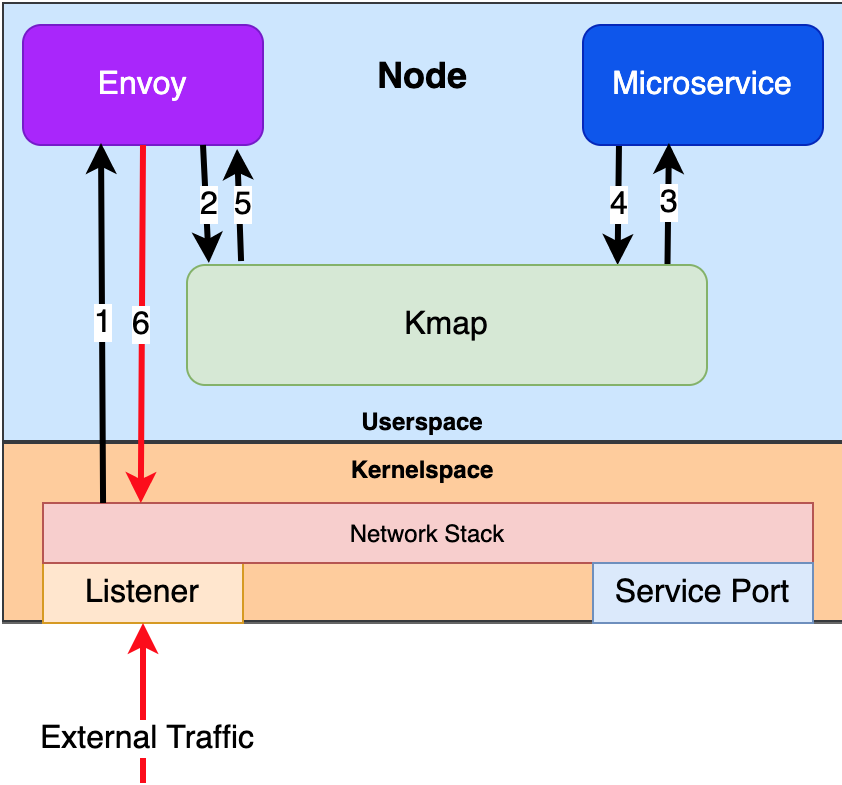
\includegraphics[keepaspectratio=true,width=3in]{figures/design/kmap.png}
        \caption{Kmap}
        \label{fig:kmap}
    \end{minipage}%
    \begin{minipage}{0.5\textwidth}
        \centering
        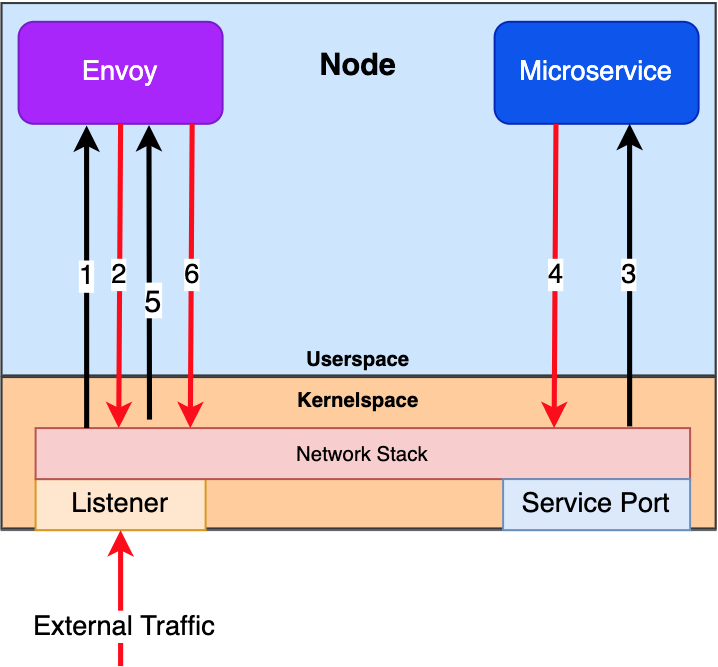
\includegraphics[keepaspectratio=true,width=3in]{figures/design/no_kmap.png}
        \caption{No Kmap Envoy Network Stack}
        \label{fig:no_kmap}
    \end{minipage}%
\end{figure*}

%\begin{figure}[!htb]
%    \begin{minipage}{0.5\textwidth}
%        \centering
%        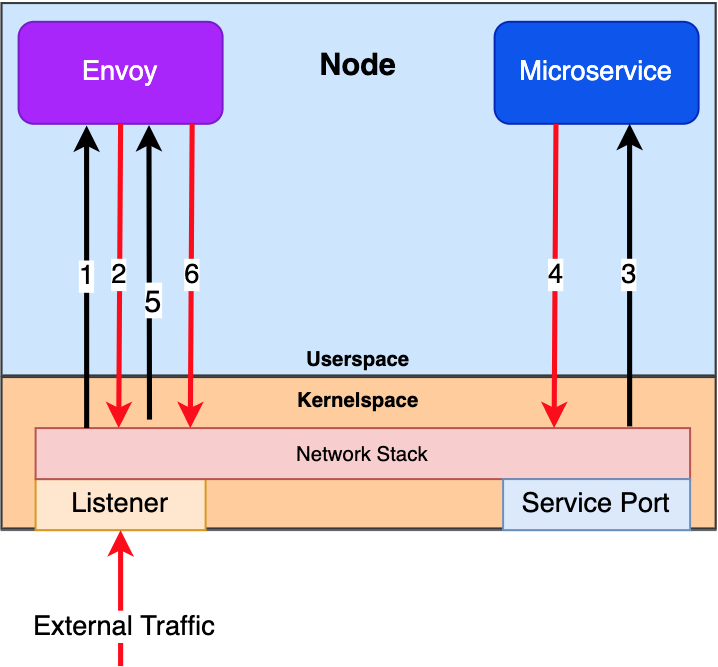
\includegraphics[keepaspectratio=true,width=3in]{figures/design/no_kmap.png}
%        \caption{No Kmap Envoy Network Stack}
%        \label{fig:no_kmap}
%    \end{minipage}%
%\end{figure}


\section{\sysname}
\label{sec:design}
Our design for \sysname focus on avoiding costly, unnecessary invocations of the network stack.
These network calls involve copying of bytes between two processes and kernel context switches.
Avoiding the extraneous copying and reducing the frequency of context switches should greatly improve data transfer speed.
Envoy prides itself on being application agnostic, which leads to the helpful ability to auto-inject Envoy into microservices.
However, this abstraction results in unnecessary invocations of the network stack.
In Figure-\ref{fig:no_kmap} we highlight in red all the calls to the network stack for the path of a single request.
Then, in Figure-\ref{fig:kmap} we show the reduction in those calls by using Kmap instead of the network stack for local data transfer.

\sysname works by using LD\_PRELOAD to load \sysname before libc regular calls.
\sysname contains several functions which match the signature of libc network calls and thus when applications invoke those calls, \sysname's version of those functions is invoked instead of libc.
Using the \sysname functions, Envoy and the microservice call read and write passing data through userspace rather than passing the data into the network stack, using shared buffers to efficiently transfer the data.
Thus, we must load the shared library for both the Envoy sidecar and the microservices.
The two critical challenges to realizing \sysname are:
\begin{enumerate}
    \item Building a robust, efficient shared buffer system that's \textit{faster} than the network stack
    \item Determining in a microservice-agnostic way which POSIX network calls should be preloaded by \sysname
\end{enumerate}

\subsection{Intercepting Network Calls}
\textbf{Direct libc Modification:}
One method of implementing \sysname would be to modify libc in environment for Envoy and the service.
This option, however, would require extensive infrastructure modification to ensuring Envoy and the service each boot with the proper libc version (compiled for them).
Further, the library change would effect any other process running the in the same environment (container or system) and thus \sysname would have to handle calls from neither Envoy or the service.

\textbf{LD\_PRELOAD:}
The Linux LD\_PRELOAD command~\cite{ldpreload} allows users to preload particular libraries ahead of the conventional linker and loader.
This enables users to load symbols before classic libraries (e.g. libc, syscalls).
Commonly this is referred to as the "LD\_PRELOAD trick"~\cite{ldtrick}.
The LD\_PRELOAD command modifies the linking process of the particular process it is attached to, requiring no modification of the default library and not interfering with any other process.


For \sysname, we use LD\_PRELOAD to load the \sysname libraries before conventional libraries such as libc.
Inside each \sysname library we use \textit{dlsym} to load the "real" libc functions we wrap.
Thus, we can use libc functions in \sysname, passing through most calls, while intercepting and adjusting only the subset relevant to \sysname.
From a maintainability perspective, this allows libc and \sysname to evolve independently while remaining compatible.

\subsection{Pipe options}
Here, we outline potential methods for implementing the buffer \sysname uses to pass data between Envoy and the microservice.

\textbf{Named Pipes:}
Named pipes, (FIFO) are blocking, uni-directional I/O buffers for passing data between two processes.
The pipe must be opened for both reading and writing before being written two.
Named pipes are traditionally slow, only offering slight speed advantages over TCP~\cite{ipcperf}.
Further, they are un-directional which makes them less accessible or interchangeable compared to TCP.

\textbf{Unnamed Pipes:}
Unnamed pipes are slightly faster than Named pipes, but are created per-process.
They traditionally are used when a process forks, as they both will share a reference to the pipe.
This makes them particularly tricky to implement across two independent processes and thus unhelpful for \sysname.

\textbf{Shared Memory:}
Shared memory is a robust API which allows processes to share use of a memory region (\textit{schm\_open}).
This requires mapping the same underlying memory region into the virtual memory of each process (\textit{mmap}).
Shared memory is concretely faster than pipes and the primary API \sysname uses for communicating information.
Shared memory has been benchmarked to be 170 times faster than TCP sockets for communicating information between processes~\cite{ipcperf}.
However, shared memory does not directly provide a buffer interface like TCP, ans so \sysname must implement that as part of its library.

\subsection{Dual Pipes}
Since \sysname mirrors the network stack for two unique clients, Envoy and the service, we must implement two circular buffers.
These buffers are unidirectional, providing read/write direction for each service.
A core function of the POSIX network stack is blocking write and reads using syscalls like \textit{select} and \textit{epoll}.
As such, we use have dedicated synchronization for each buffer using pthread mutexes and conditional variables.
We display these aspects of \sysname in Figure-\ref{fig:closeup}


\begin{figure}[!htb]
    \begin{minipage}{0.5\textwidth}
        \centering
        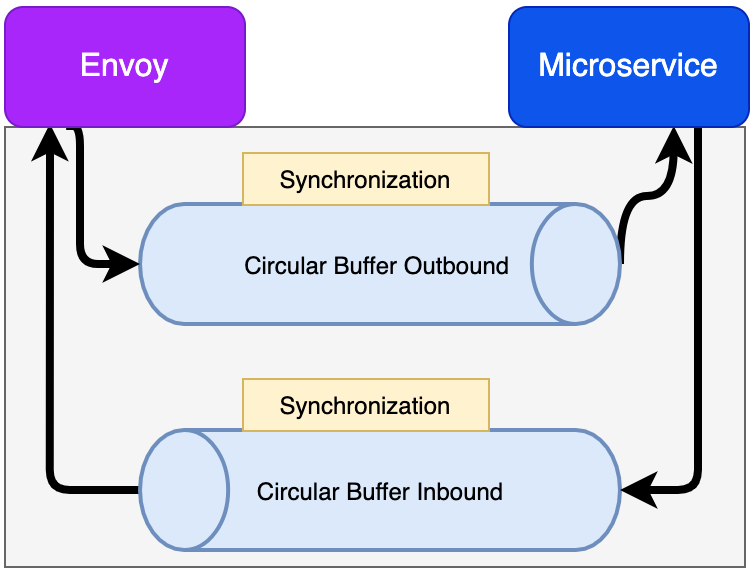
\includegraphics[keepaspectratio=true,width=3in]{figures/design/kmap_closeup.png}
        \caption{Kmap Design}
        \label{fig:closeup}
    \end{minipage}%
\end{figure}

\subsection{When to apply \sysname}
The network stack has a very well defined, robust API commonly called POSIX sockets.
A particular challenge for \sysname is pre-loading in front of these network calls and knowing when
to pass through the call, or when to route to the local buffer.
Since \sysname is designing primarily for Envoy, we use information about how it communicates with microservices to determine which file descriptors should use \sysname.
The Envoy codebase uses unique handlers for different requests (e.g. gRPC, TCP, HTTP 2, HTTP 3, QUIC) and as such \sysname will have to adjust it's structure to match the protocol in use.
For now the focus of our \sysname prototype, discussed in Section-\ref{sec:prototype} is Envoy's HTTP stack.
We do not view \sysname as generalizable to other Envoy paths or other tools (e.g. Linkerd) without thorough inspections of the pathways.
It is likely for \sysname to generalize it would require the tool and path as part of its compilation process.


\section{Prototype}
\label{sec:prototype}
Here, we discuss our current prototype, challenges, and target applications.
Currently we compile a single shared object (\{envoy,service\}.so) for each side using compiler flags.
It is imperative we intercept syscalls on each side, and as such we must know which side of communication the library is running on to determine which network calls to intercept.
Our library is written in C and is approximately 800 LOC.

\subsection{\sysname Buffer}
The implementation started with named pipe as the main IPC mechanism.
However, due to its unidirectional nature and difficulty in incorporating synchronization mechanisms, we decided the named pipes will not suffice.

As a solution, we used \texttt{shm\_open(2)} to open a file descriptor associated with a region of shared memory and mapped it to the process using the \texttt{mmap} syscall. We allocated a circular buffer of size $2^{24}$ bytes in this shared region and read and write from it directly using \texttt{memcpy}. We will discuss our choice of the buffer size and how it affects the performance in later section. We allocated two such buffers to provide communication in each direction.

\subsection{Concurrency Challenges}
The Envoy process will write the outer request to the buffer and read the service response from the buffer; the service process will read the request (passed on by Envoy) and write the response, as returned by the service.
We now have a classic producer-consumer problem.

Our first attempt at the solution was semaphore.
We allocated two semaphores, each associated with one buffer, for the purpose of waiting and notifying.
However, semaphores did not provide a convenient way to guarantee exclusive access to the buffer.
This allowed for data races and caused the program to malfunction.

As an improvement, we moved to using mutexes across processes.
Each buffer has a mutex associated with it and also a condition variable.
We use these two constructs to guarantee mutual exclusion and to solve the consumer-producer problem.


\begin{table}[!ht]
    \begin{center}
        \resizebox{0.5\columnwidth}{!}{
            \begin{tabular}{ |c|c|c|}
                \hline
                \textbf{Function} & \textbf{Envoy} & \textbf{Service} \\
                \hline \hline
                connect & X &  \\ \hline
                accept &  & X \\ \hline
                write & X & X \\ \hline
                read & X & X \\ \hline
                writev & X &  \\ \hline
                readv & X &  \\ \hline
            \end{tabular}
        }
        \caption{Libc Functions Preloaded (Tiny C Webserver)}
        \label{t:libraries_cserver}
    \end{center}
\end{table}

\subsection{\sysname Network Calls}
The most challenging aspect of \sysname's design is properly intercepting and replicating the behavior of network system calls.
This aspect is especially challenging because Envoy uses unique handlers for request types (UDP, TCP, HTTP\{1,2,3\}, gRPC, Quic).
Further, the service itself may use the network stack in obtuse ways.
To make \sysname generalizable, one would truly have to intercept every network call (or possible network related).

This task is enormous.
Take for example, how services often take advantage of configurable aspects of the network stack like \textit{setsockopt}.
Setting options on a particular socket changes the behavior of accept, i/o, and more.
For example, our investigation of Flask~\cite{flask} revealed that it does not call \textit{accept} for new connections.
Thus, for \sysname to properly mirror the POSIX API to services in an agnostic way, it would have to model the entire state diagram for sockets.

For our prototype we have focused on HTTP. In our prototype, a service user would contact Envoy with an HTTP GET request.
Envoy uses \texttt{readv} and \texttt{writev} in order to read from and write to multiple file descriptors at the same time.
Our tiny C server\cite{tiny} uses low level file IO system calls (e.g. \texttt{read} and \texttt{write}).
We summarized the intercepted network syscalls in Table-\ref{t:libraries_cserver}.


\subsection{Initialization}\label{subsec:initialization}
We use the GCC feature \textit{\_\_attribute\_\_((costructor))} to tell GCC to compile our library such that before any functions are invoked we can load kmap.
The memory allocation can take a second or two depending on the size of memory allocated.
Thus, we run initialization/mapping functions for each side via the constructor, rather than on invocation.
This also helps optimize performance by not requiring runtime initialization checks on the functions.

\begin{figure}[!htb]
    \begin{minipage}{0.5\textwidth}
        \centering
        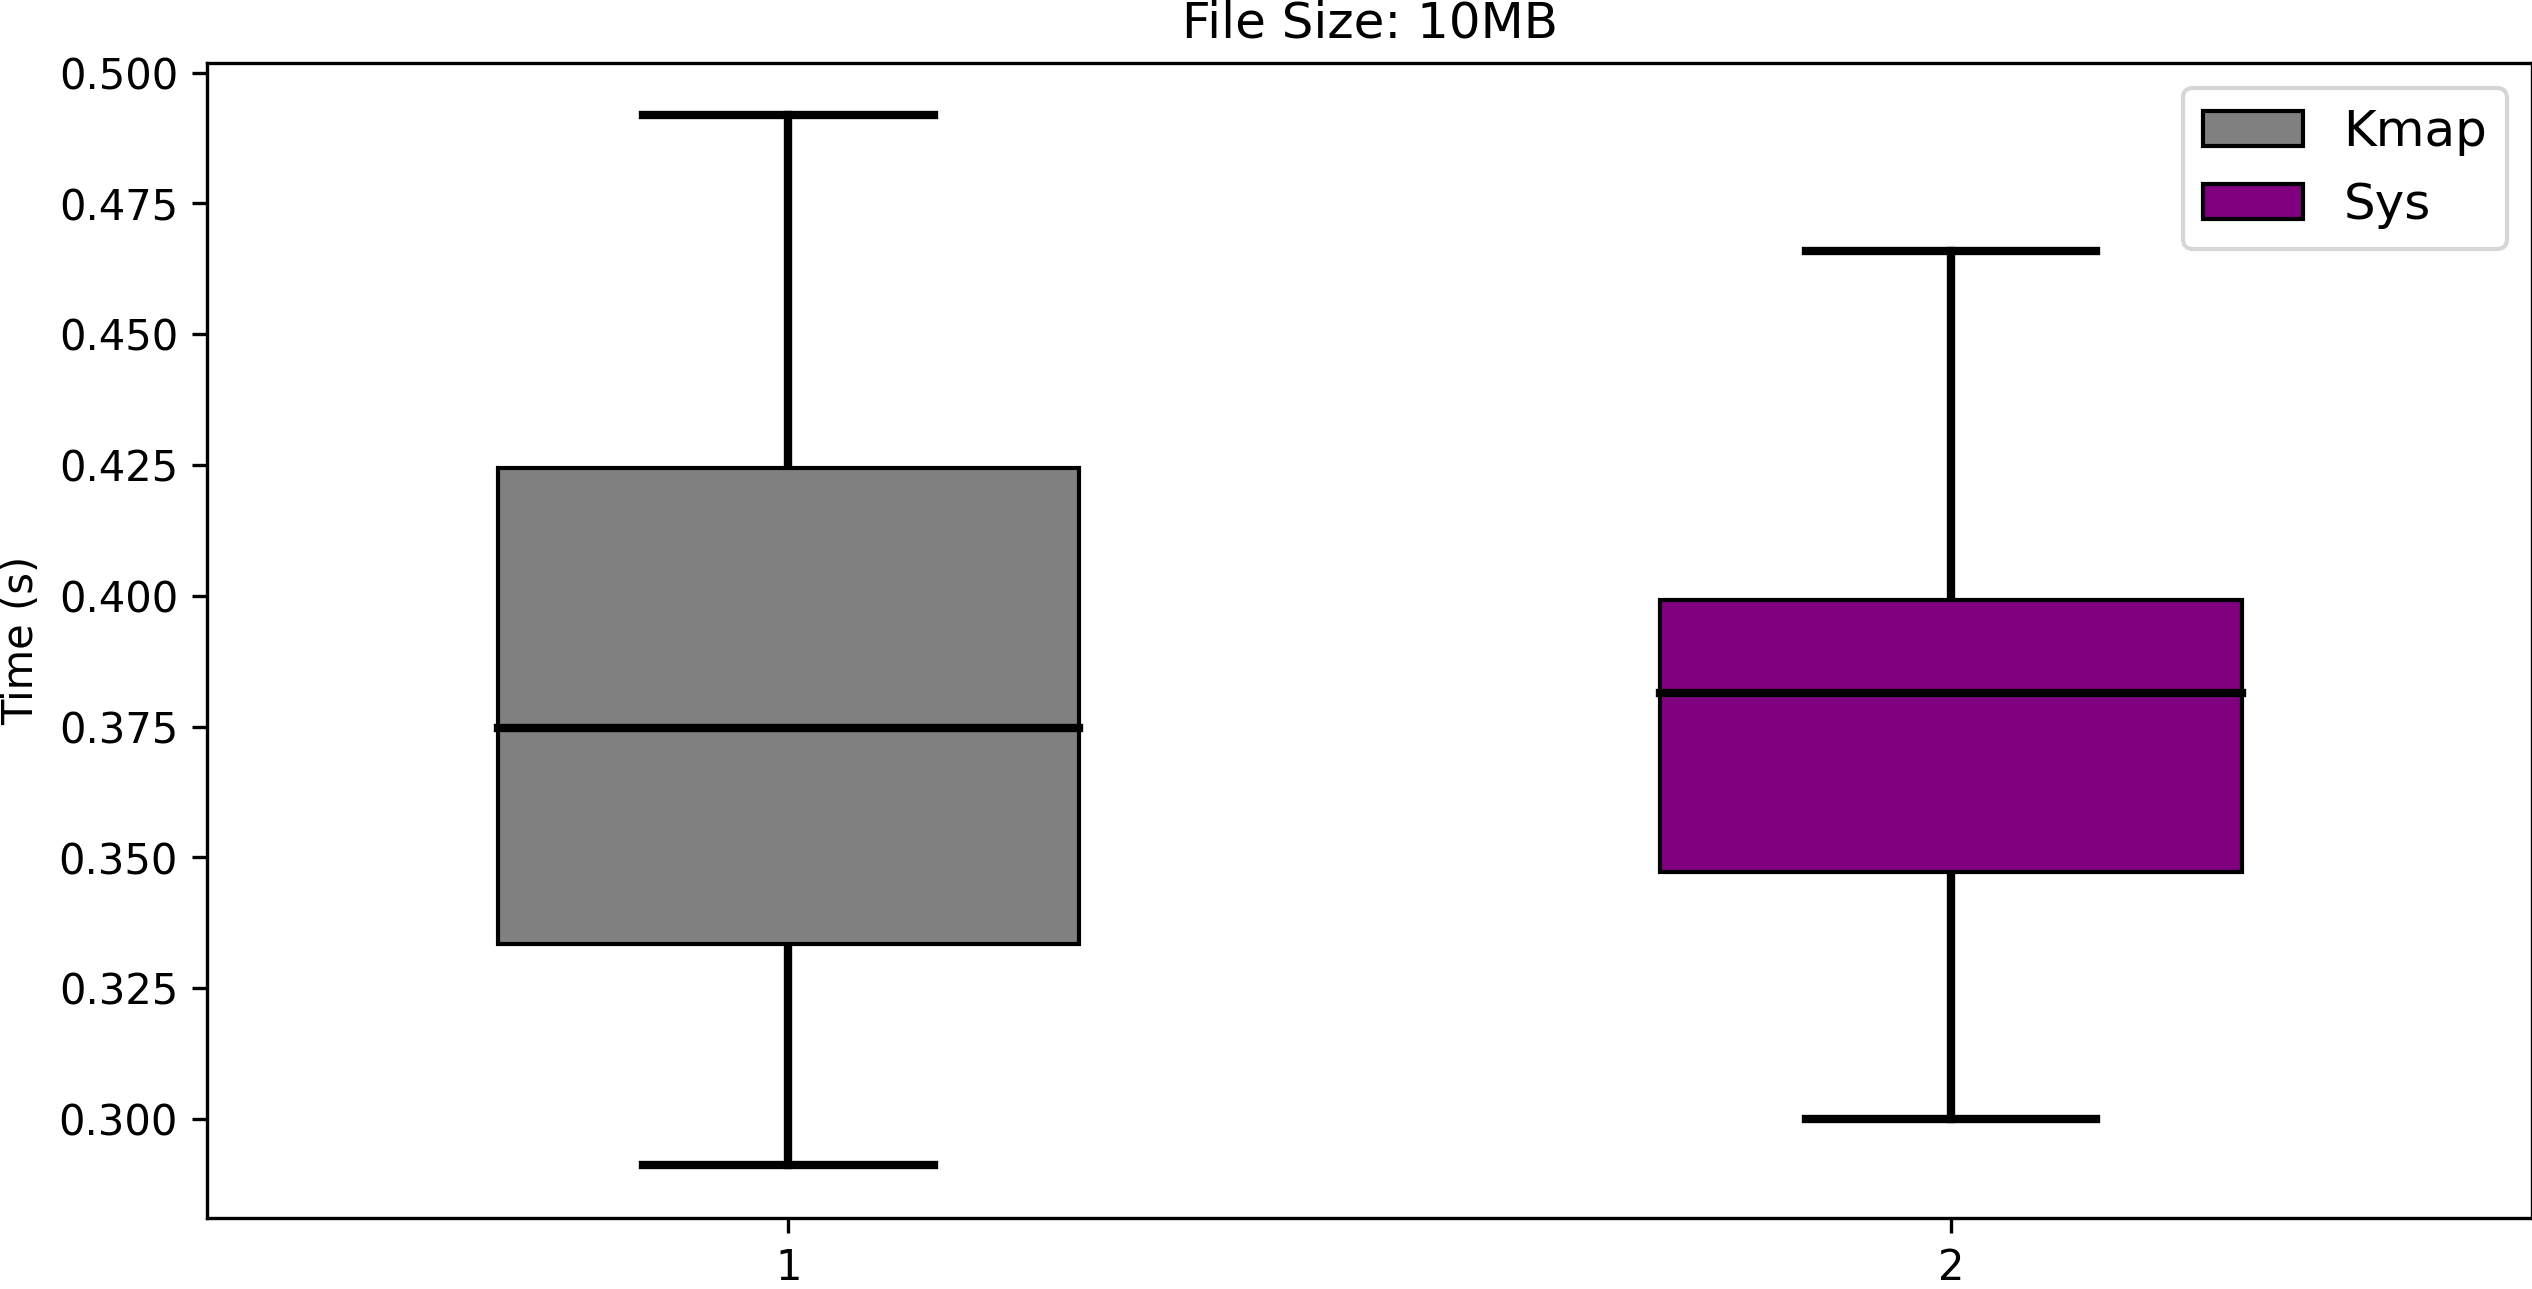
\includegraphics[keepaspectratio=true,width=3in]{figures/evaluation/netload.png}
        \caption{\sysname with Network Under Load}
        \label{fig:netload}
    \end{minipage}%
\end{figure}


\begin{figure*}[!htb]
    \begin{minipage}{0.5\textwidth}
        \centering
        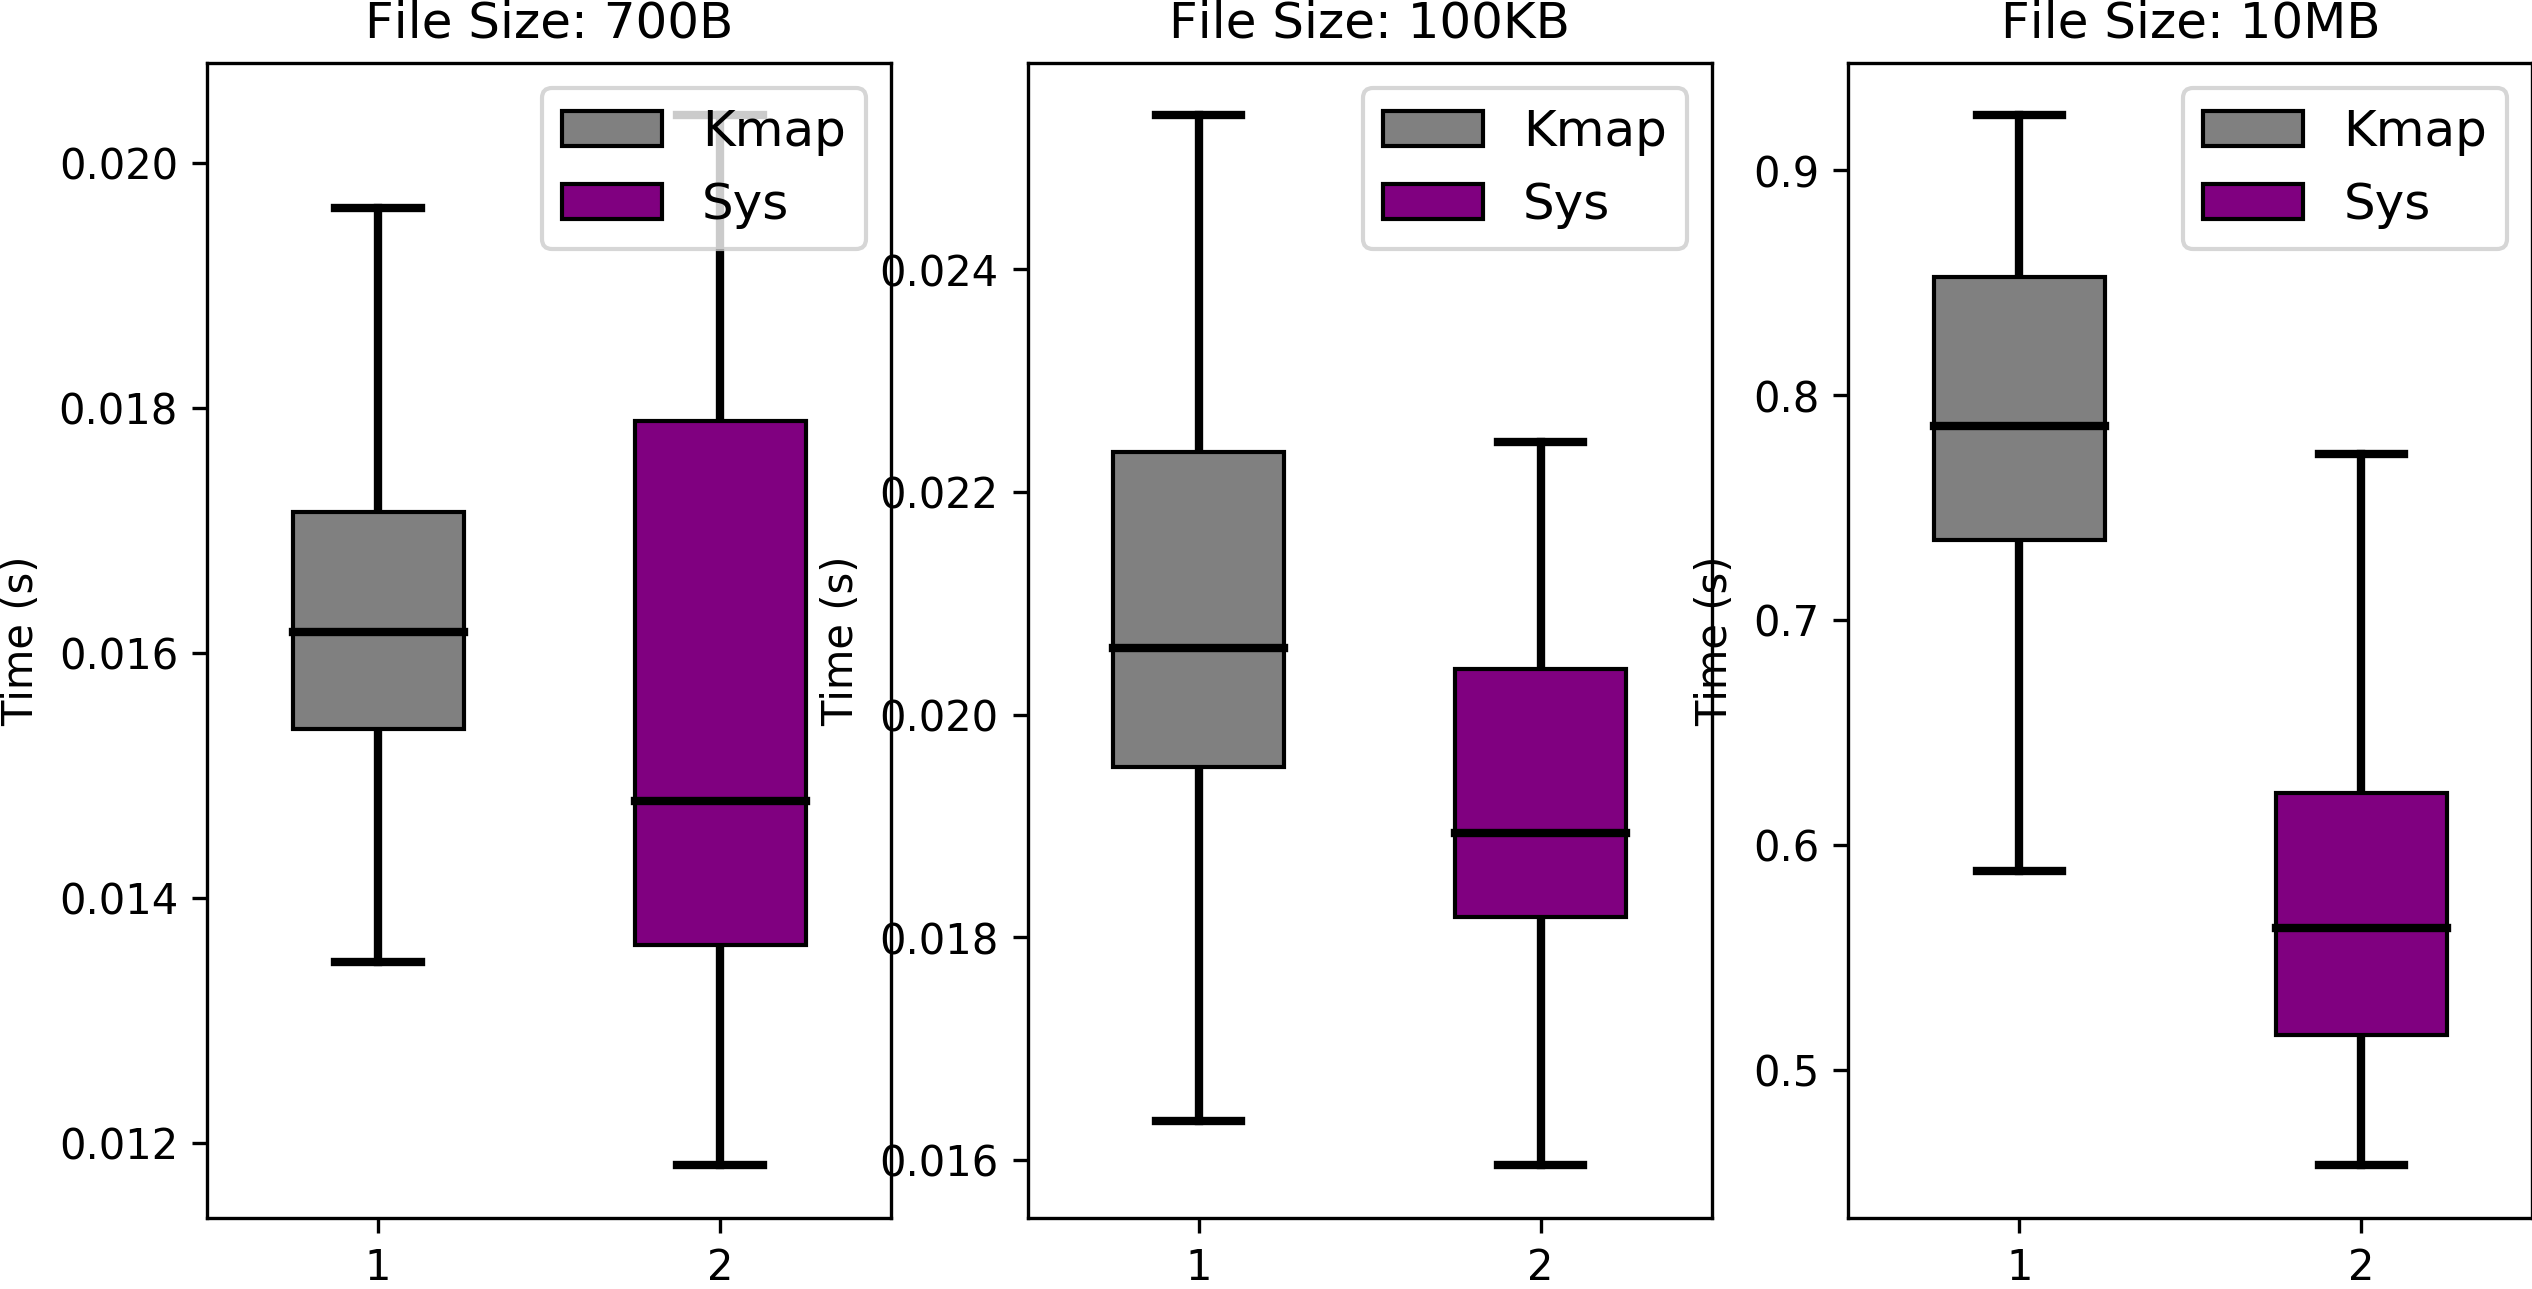
\includegraphics[keepaspectratio=true,width=3in]{figures/evaluation/results.png}
        \caption{Time to Transfer}
        \label{fig:results}
    \end{minipage}%
    \begin{minipage}{0.5\textwidth}
        \centering
        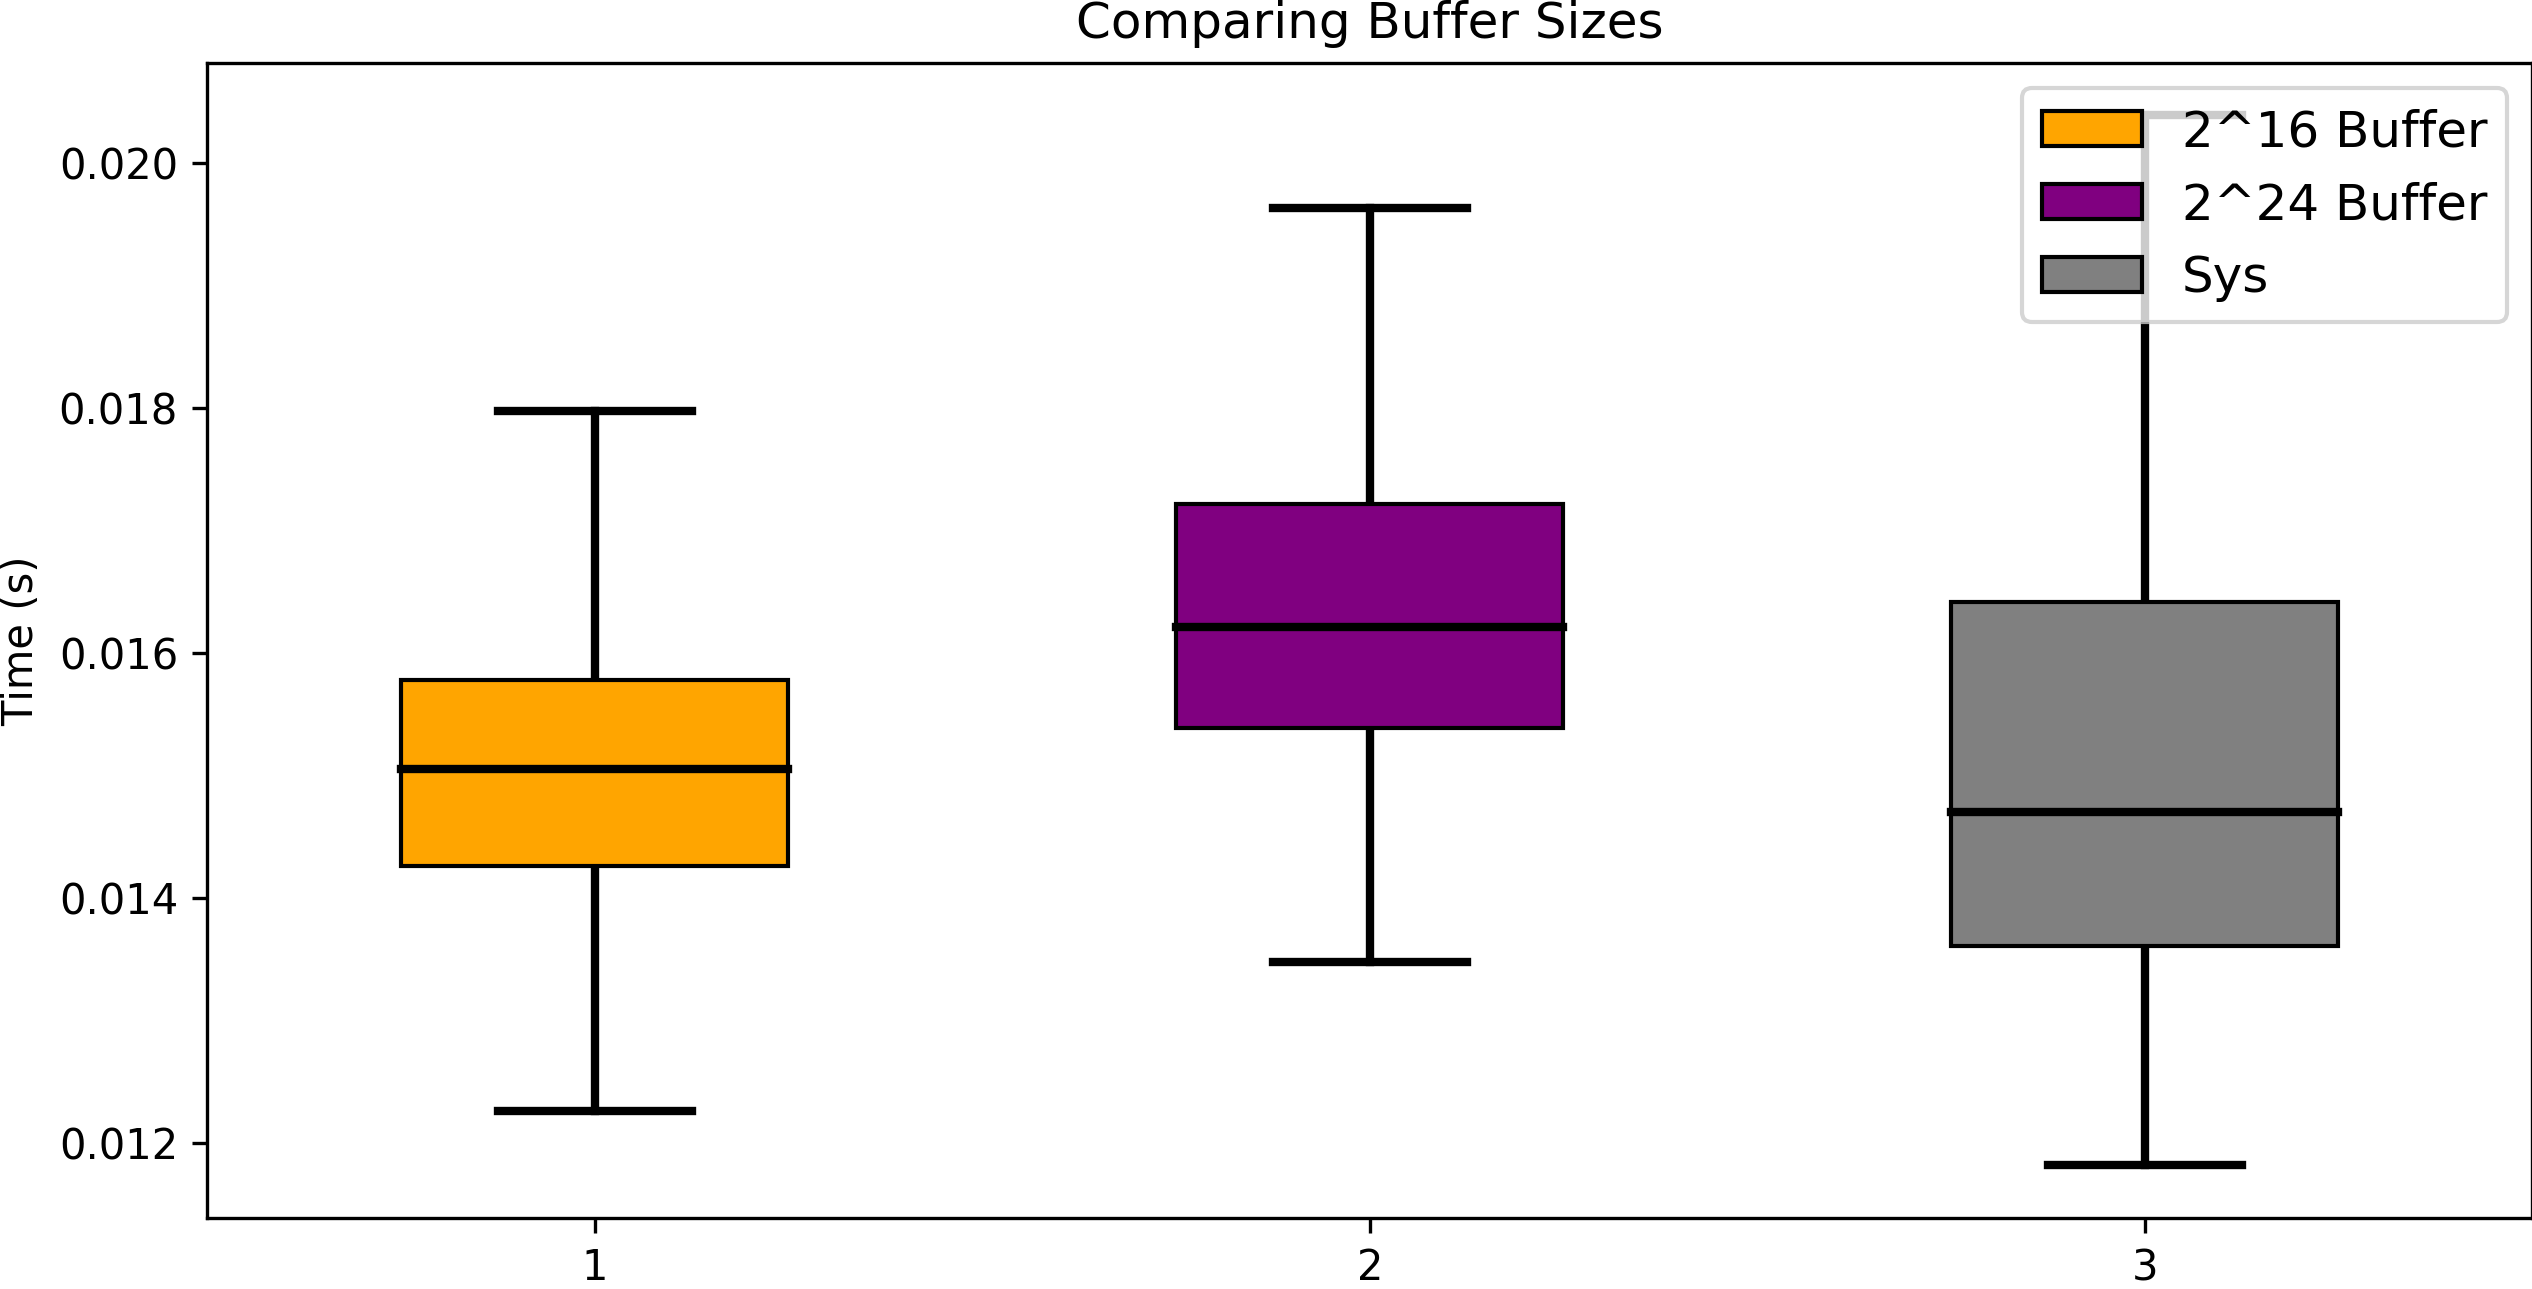
\includegraphics[keepaspectratio=true,width=3in]{figures/evaluation/buf_compare.png}
        \caption{Comparing \sysname Buffer Sizes}
        \label{fig:buf}
    \end{minipage}%
\end{figure*}
\section{Evaluation}
\label{sec:evaluation}
\textbf{Experimental Design}:
We tested \sysname by running a single docker container with Envoy and our Tiny C Webserver~\cite{tiny}.
We then issue a series of programmatic requests to the container, targeting the Envoy port which in turn returns the content from the webserver.
We generally served fixed size randomly generated byte files, which we then compared on delivery to confirm efficacy.

\subsection{General Performance}
Our first test compares the time to transfer of 3 different size files 700B, 100KB, and 10MB.
In this experiment we use a buffer of $2^{24}$ bytes, which can support all the files.
Our results are shown in Figure-\ref{fig:results}.
We see that with smaller files \sysname is on par with the default system performance.
At higher file sizes \sysname falls behind.
Our hypothesis here is that Envoy uses readv to read data out of the buffers into iovectors.
Thus, larger files require a large number of reads, and, under the assumption our read compared to the system read is slower, this compounds \sysname's time increase.

\subsection{Buffer Size}
Our next experiment evaluated the performance of different buffer sizes.
We looked at the time to transfer for the tiny file across 2 buffer sizes $2^{16}$ and $2^{24}$ and compare those times to the system.
The results, shown in Figure-\ref{fig:buffer}, showed that the $2^{16}$ Byte buffer performed better.
We believe this is because the smaller buffer requires less pages and the memory may be more closely located since the process is not requesting as large a chunk.

\subsection{Busy Server}
Our previous two experiments were run in isolation without any other running processes.
For the majority of microservice deployments this is not representative of the typical workload.
Thus, our next experiment simulates concurrent usage.
We ran a netcat TCP stream at 5MB/s on the same node as our \sysname test.
Our finding is summarized in Figure-\ref{fig:netload}. Although our result shows some fluctuation, which is a problem that certainly should be revisited in the future, the median and minimum both surpassed what the Unix domain sockets achieved.
The cost of kernel operations is increased when other processes are using the network stack as well, as now the kernel must handle multiple network connections at the same time.
Further, this test more closely resembles real-world deployment and thus we are optimistic that \sysname's principles remain strong.


\section{Related Work}
In this section, we highlight work with a similar goal or method to \sysname.
In this, we hope to show that \sysname has taken inspiration from existing network tools and is rooted in a growing body of work.

\textbf{NetKernel:~\cite{netkernel}}
This work focuses on moving optimizing the network stack by moving it out of the kernel.
The impetus was in the VM-age, riping the kernel out of the VM itself provides more control and optimization for users.
Their improvements include shared memory.
In their work (Section 4.1) they discuss the use of LD\_PRELOAD for transport socket redirection.
For their usecase, LD\_PRELOAD was not robust enough and required too many mappings.
However, we see that for \sysname the transport socket redirection should be sufficient.


\textbf{Slim (OS):~\cite{slimos}}
SlimOS addresses performance challenges within the container network stack.
Similar to \sysname, they attempt to avoid traveling the virtualized network stack and directly preceding through the host network interface.
They work works at a lower abstraction level than \sysname but employs a similar principal.
SlimOS dynamically links its user-space library onto of containers using LD\_PRELOAD on unmodified application binaries.


\textbf{Grafting Sockets:~\cite{graft}}
This work expands a new socket option AF\_GRAFT to optimize container networking.
They expanded POSIX sockets to include the new option, allowing applications to build directly with it.
Additionally, they use LD\_PRELOAD to load the AF\_GRAFT library without any application modification.


\textbf{clARMOR:~\cite{clarmor}}
clARMOR uses LD\_PRELOAD to load a buffer-overflow detection library.
The tools highlights the applicability and widespread use of LD\_PRELOAD for injecting additional logic into system class without requiring application modification.
\section{Discussion}
\label{sec:discussion}
Our work in Section-\ref{sec:evaluation} shows \sysname is comparable to the default system in certain circumstances and performs better in a select few.
Throughout our process, we attempted a number of optimizations which generally did not have much effect.
We will highlight them here and explain why we view that they were inconsequential.
We will also discuss future directions and learnings from the project.

\subsection{Optimizing \sysname}
Our results show the end of a number of improvements we made to \sysname.
Though no individual improvement significantly adjusted \sysname's performance.

\textbf{Compiler:} Our work began by writing the library with no compiler optimization.
Compiling with optimization flags of 02 or 03 did not adjust performance much.
The code base is relatively small and low-level so we did not expect much improvement.
Nevertheless running compile optimized code is a good practice.


\textbf{Copying:} We also experimented with the way we copied bytes.
Our naive first implementation copied at the byte level in and out of the buffer.
We improved this by using \textit{memcpy} and even experimented with multithreading \textit{memcpy}.
In either case, the improvement we saw was minimal, leading us to our cumulative conclusion that the network stack is highly optimized.

\textbf{Unsafe execution:} Another method of optimization we took was to avoid error checking in the main path of function calls.
By this, we mean that we don't null check or offset check as much as is possible.
We moved much of our initialization to the library constructor and assume it is run first (start up takes < 1 second).
The improvement this technique provided was very slight.

Overall, we feel that these optimizations were relatively surface-level.
By this, we mean that they all improve the way we communicate with our shared memory and the other processes.
They do not \textit{themselves} optimize shared memory, where we feel is causing the slow-down.

\subsection{Next Steps and Lessons}
We feel that the work here shows \sysname's promise.
Further evaluation and exploration are needed to understand under which environments \sysname performs better.
Further paths (i.e TCP/UDP/gRPC) also may show different results.
Ultimately, though, we view that this confirms how optimized the network stack is.
In principle, \sysname should be a streamlined version of the network stack, however, the decades of work built in to the kernel cannot be unappreciated.





\bibliographystyle{acm}
\bibliography{paper}

%%%%%%%%%%%%%%%%%%%%%%%%%%%%%%%%%%%%%%%%%%%%%%%%%%%%%%%%%%%%%%%%%%%%%%%%%%%%%%%%
\end{document}
%%%%%%%%%%%%%%%%%%%%%%%%%%%%%%%%%%%%%%%%%%%%%%%%%%%%%%%%%%%%%%%%%%%%%%%%%%%%%%%%

%%  LocalWords:  endnotes includegraphics fread ptr nobj noindent
%%  LocalWords:  pdflatex acks
